\documentclass[11pt]{article}
\usepackage{geometry}                
\geometry{letterpaper}                   


\usepackage{hyperref}
\usepackage{color}

\usepackage{graphicx}
\usepackage{amssymb}
\usepackage{epstopdf}
%\usepackage{natbib}
\usepackage{amssymb, amsmath}
\DeclareGraphicsRule{.tif}{png}{.png}{`convert #1 `dirname #1`/`basename #1 .tif`.png}

\title{Opinion Formation: Impacts of convincing extreme //
individuals onto a society that typically converges to one opinion}
\author{Alexander Stein, Niklas Tidbury, Elisa Wall}
\date{date} 

\begin{document}



\thispagestyle{empty}

\begin{center}

\includegraphics[width=5cm]{ETHlogo.eps}

\bigskip


\bigskip


\bigskip


\LARGE{ 	Lecture with Computer Exercises:\\ }
\LARGE{ Modelling and Simulating Social Systems with MATLAB\\}

\bigskip

\bigskip

\small{Project Report}\\

\bigskip

\bigskip

\bigskip

\bigskip


\begin{tabular}{|c|}
\hline
\\
\textbf{\LARGE{Insert Title Here}}\\
\textbf{\LARGE{...}}\\
\\
\hline
\end{tabular}
\bigskip

\bigskip

\bigskip

\LARGE{Name 1 \& Name 2}



\bigskip

\bigskip

\bigskip

\bigskip

\bigskip

\bigskip

\bigskip

\bigskip

Zurich\\
May 2008\\

\end{center}



\newpage

%%%%%%%%%%%%%%%%%%%%%%%%%%%%%%%%%%%%%%%%%%%%%%%%%

\newpage
\section*{Agreement for free-download}
\bigskip


\bigskip


\large We hereby agree to make our source code for this project freely available for download from the web pages of the SOMS chair. Furthermore, we assure that all source code is written by ourselves and is not violating any copyright restrictions.

\begin{center}

\bigskip


\bigskip


\begin{tabular}{@{}p{1cm}@{}p{5cm}@{}@{}p{5cm}@{}@{}p{5cm}@{}}
\begin{minipage}{1cm}

\end{minipage}
&
\begin{minipage}{5cm}
\vspace{2mm} \large Alexander Stein

 \vspace{\baselineskip}

\end{minipage}
&
\begin{minipage}{5cm}

\large Niklas Tidbury

\end{minipage}
&
\begin{minipage}{5cm}
	
	\large Elisa Wall
	
\end{minipage}
\end{tabular}


\end{center}
\newpage

%%%%%%%%%%%%%%%%%%%%%%%%%%%%%%%%%%%%%%%



% IMPORTANT
% you MUST include the ETH declaration of originality here; it is available for download on the course website or at http://www.ethz.ch/faculty/exams/plagiarism/index_EN; it can be printed as pdf and should be filled out in handwriting


%%%%%%%%%% Table of content %%%%%%%%%%%%%%%%%

\tableofcontents

\newpage

%%%%%%%%%%%%%%%%%%%%%%%%%%%%%%%%%%%%%%%



\section{Abstract}

\section{Introduction and Motivations}
For millennia, society has consisted of many opinions and points of view. In some cases, these opinions have been oppressed, other opinions have been forced onto societies, others brainwashed. Within a democracy, these opinions are given space to spread, to change and to evolve and yet: they still converge into a general opinion. How is this possible in cases of extremism, where extreme opinions are so different compared to the majority? What effect do extreme opinions, such as that of the IS, Charles Manson and Co. have on a converging opinion of a society? We would like to examine how extreme opinions of individuals impacts such a society, and under what circumstances these opinions can have a wide-spread effect. \\*
Basing on the papers of Holme and Newman \cite{Coevolutions} such as Laguna, Abramson and Zanette \cite{Minor}, a socienty of opinions in the range [0,1] converges against an average opinion 0.5 if the parameters are set accordingly. To make it easier, we started from that situation and added the extreme opinion people in order to see how it affects the outcome. \\*
Our questions are basically the following: 
\begin{itemize}
\item What are the outcomes of n convincing individuals of extreme opinions in a society that converges to one opinion? Do we see fragmentation or polarisation of opinions?
\item What effects do these extreme opinions have in a society of low $u$ [narrow communicating interval] and $\mu$ [weight of foreign opinions]?
\item What happens when we vary the random distribution?
\end{itemize}


\section{Model and Implementation}
\subsection{Society agent in a single time step}
We have set a society of $N$ agents with opinions $x_i \in [0,1]$, $i \in \{1, N \}$. Initially the distribution of opinions is uniform, which means that all opinions are equally alike.

We further define the parameter of a threshold of communication $u$. So agents interact with each other only if their difference in opinion is smaller than this threshold. In \cite{Minor} this is introduced as the "bounded confidence" which corresponds to the fact that people tend to spend time with agents with similar opinion, for instance circle of friends tend to be of similar opinion. By building a threshold u into the structure, the agents only interact with similar-thinking agents, as people generally interact with the like-minded. A big $u$ therefore corresponds to open-minded society agents which interact with people of an opinion "further away".

The second parameter is the $\mu$, which represents the weight on other opinions of each society agent. When two agents interact with each other they mutually adapt their opinion to some opinion in the middle. \\

The concrete implementation as in \cite{Minor} looks as follows:
\begin{equation}
\begin{aligned}
x(t+1) &= x(t) + \mu(x'(t) - x(t))  \\
x'(t+1) &= x'(t) + \mu(x(t) - x'(t)) 
\end{aligned}
\end{equation}

Note that only weight adjustments $0 < \mu < 1$ are allowed to guarantee that the opinions after are between the two initial opinions and that the values do not exceed the range of [0,1]. A negative value would mean that opinion of the two agents would develop in the opposite direction of opinion. \\*
A characteristic property of this model is the fact that close opinions come even closer and opinions further away from each other do not influence each other, whereby "close" and "far-away" are defined by $u$. \\*
Up to now we have defined under which threshold two agents meet and under which weight they exchange their opinion. The next point is to define a single time step in such a way that every agent randomly chooses another agent within the society and the threshold of communication $u$ to interact with him as described above. Then we iterate over the $T$ time steps to get the final update of opinions.
As concluded in \cite{Minor}, first of all the parameters $\mu$ and $T$ are related in such a way that the results at given $u$ do not vary if by reducing one the other has to be increased. If moreover a high enough value of $u$ = 0.3 or greater as a communication threshold is chosen, the society's opinion converges to a unique opinion around $x$ = 0.5.

\subsection{Extremists}
Basing on the setting of society of interacting agents with the three parameters $u$, $\mu$ and $T$ of the last chapter we add extreme individuals of non-changing opinion on each of the outskirts of the opinion range at 0 and 1. They represent charismatic individuals of good rhetorics able to convince a lot of people on their opinion, such as social media stars or politicians with extreme opinions. \\*
This is implemented with the following parameters for each of the two sides: At each time step the $n$ extreme opinion individuals can persuade $p$ other agents by a probability of success of $\kappa$ each, but again only within a threshold of communication, this time called $infop$. \\*
So here we seemingly add four new parameters to $u$, $\mu$ and $T$, but in fact there are some correlations, just as there were correlations between $\mu$ and $T$ in the case without extremists.
Firstly, we have an effective number of persuaded people in each time step of $n_{eff} = n \cdot p$ that and that can be united as one parameter. Secondly, this again then can be united to $n_{conv}$ = $\kappa \cdot n_{eff}$, under {\color{red}the constraint that we have high enough numbers such that statistical averages take place}. \\*
So in the end we have only two additional parameters $n_{conv}$ and $infop$ in the case of the society with extremist, with a total of five parameters of $u$, $\mu$, $T$, $n_{conv}$ and $infop$.

\section{A world without extremists}
In order to keep things easier, we started the simulations with a society without extremists converting against a common opinion around $x$ = 0.5. We therefore first had to code a situation as given in \cite{Minor} in order to reproduce the results.

\subsection{The weight \texorpdfstring{$\mu$}{TEXT} gives the speed of convergence, but has no influence on result}
We reproduce the fact, that $\mu$ only acts as a parameter of convergence, and that in the case of a constant $u$ a small $\mu$ has to be compensated with a high number of time steps $T$ and that the results are the same apart from that.

\begin{figure}[!htb]
\minipage{0.32\textwidth}
  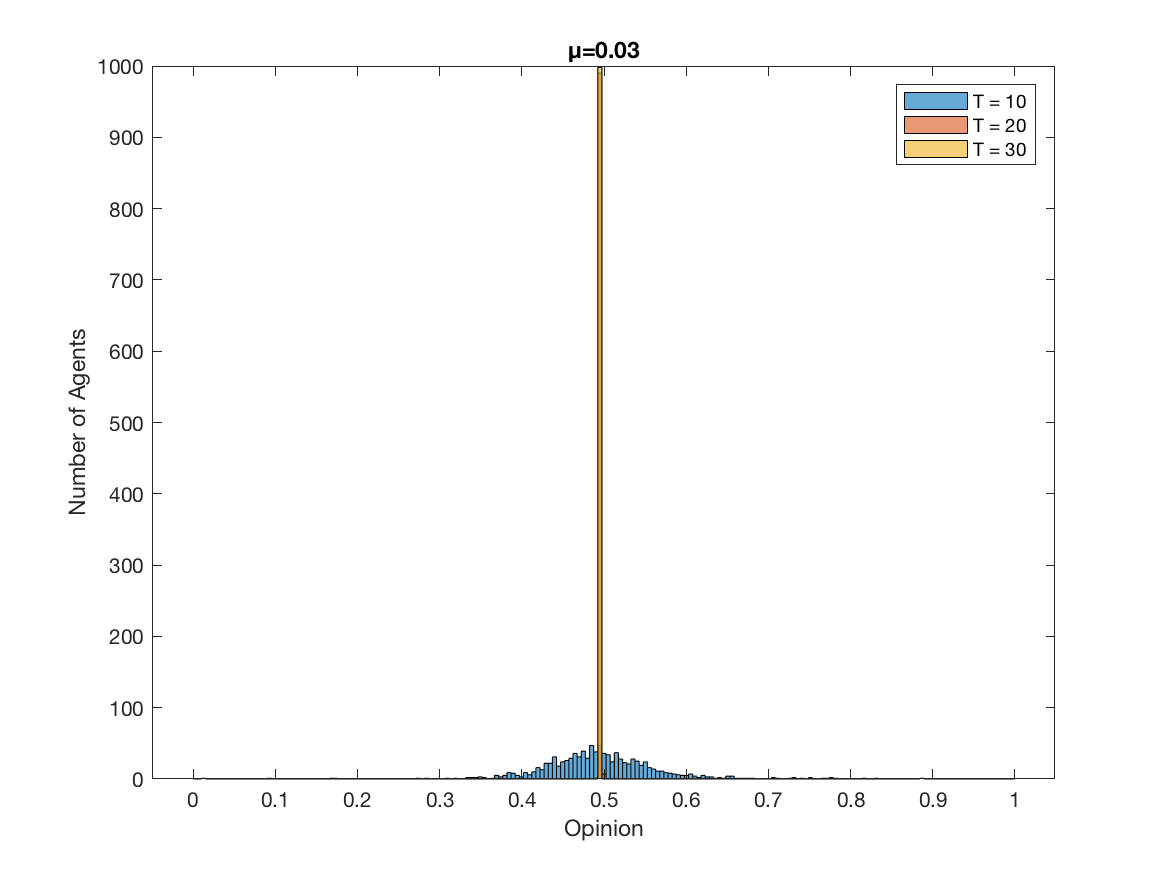
\includegraphics[width=\linewidth]{gen_plot_2017121415381080438e+01.png}
\endminipage\hfill
\minipage{0.32\textwidth}
  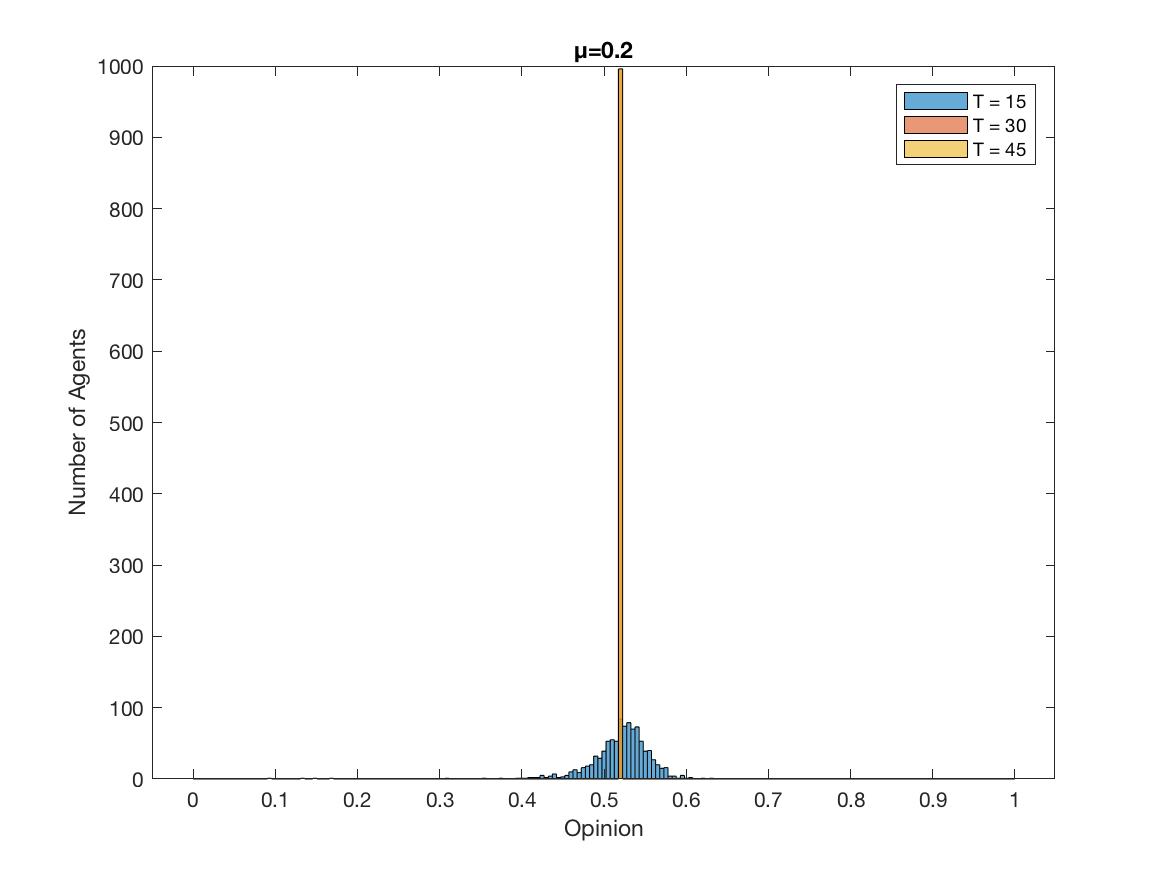
\includegraphics[width=\linewidth]{gen_plot_2017121415383200164e+00.png}

\endminipage\hfill
\minipage{0.32\textwidth}%
  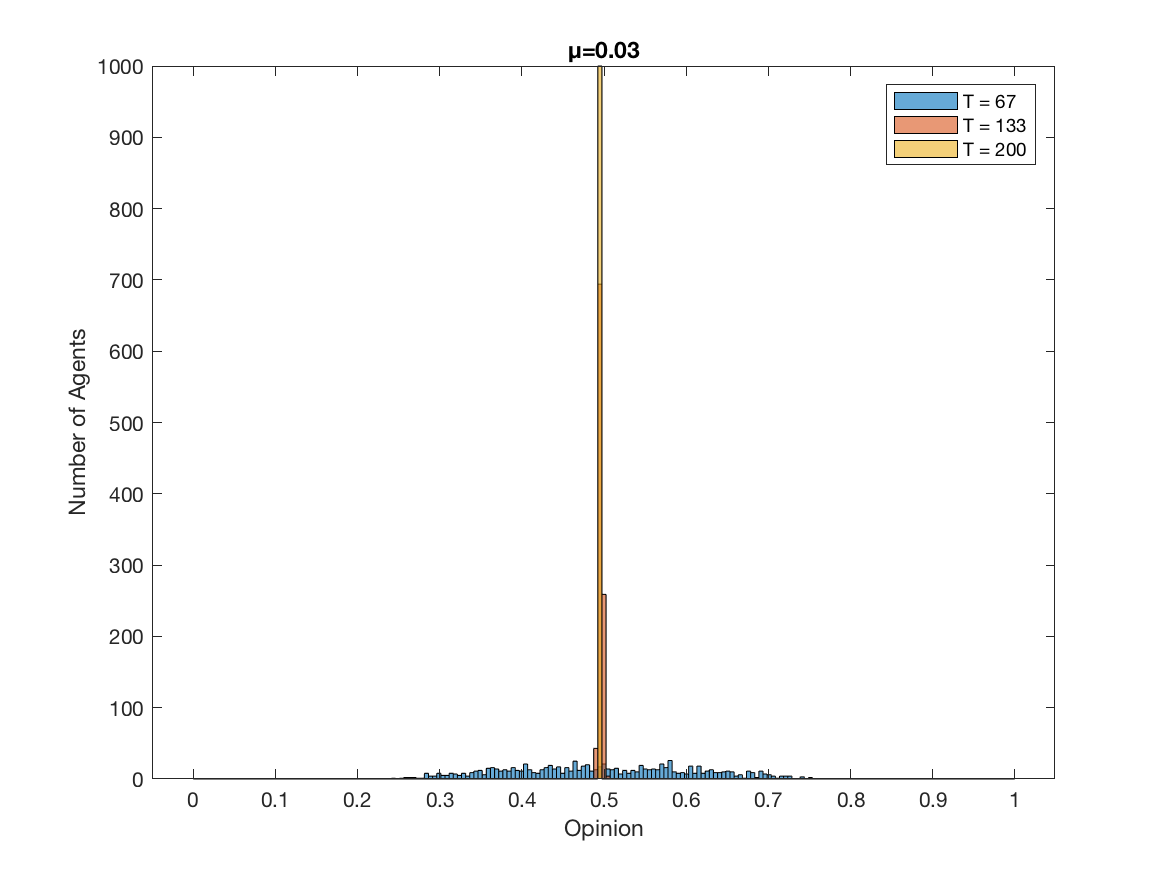
\includegraphics[width=\linewidth]{gen_plot_2017121415386231505e+00.png}
\endminipage
\label{fig:muwithoutextremists}
\end{figure}


\subsection{The threshold u defines the cluster building}
According to \cite{Minor}, such a society of N agents with random uniform distributed opinions $x_i$ in [0,1] will converge to a common opinion around 0.5 if the comunicating interval $u$ of agents communicating with each other is big enough, more precise if $u>0.3$.
\begin{figure}[!htb]
  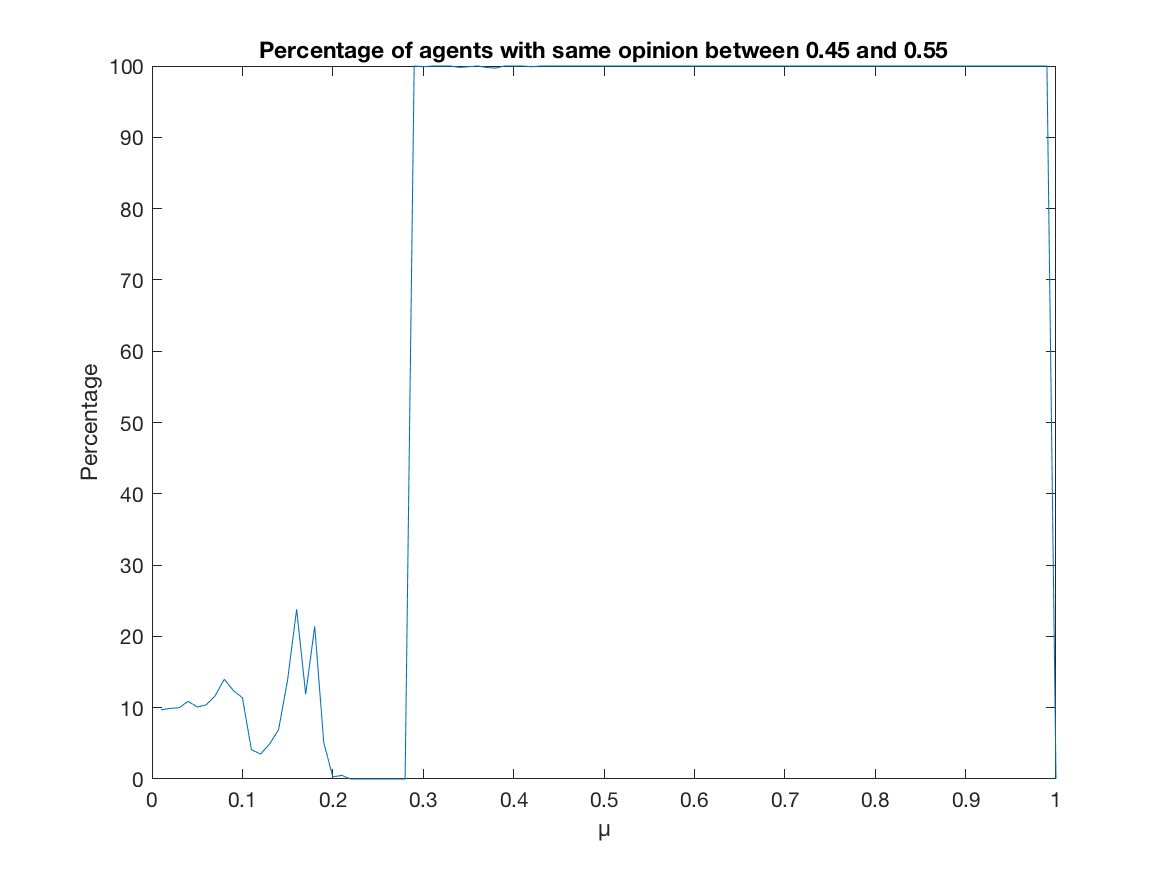
\includegraphics[width=0.6\linewidth]{gen_plot_intervall_2017121415382179938e+01.png}
\end{figure}

\section{A world with extremists}
The society model described above is being extended to a society with extreme opinion individuals who can influence the agents. We carry on to vary different parameters in this society model.
\subsection{Varying weight \texorpdfstring{$\mu$}{TEXT}}
In the case of a society without extremists, $\mu$ was just a measure of convergence, but did not have an influence on the result. So if a small $\mu$ was chosen, we number of timesteps T could be increased accordingly to get  to the same result of convergence (See Chapter 4.1). \\*
While varying the values of $\mu$ and T in a society with extremists, $/mu$ does not only influence the convergence, but also the spread of opinions. If a small $\mu$ is chosen, thus the natural convergence is slow, this leads to more agents with extreme opinions, compared to a high $\mu$. \\*
This can be explained as follows: If the natural convergence is slow, more time steps are needed to get to the stationary state. But the extremists influence is independent of $\mu$. Therefore, if the natural influence is small, the extremists have more time to grasp agents with opinions in the interval accessible to the the agents who could pull them to the average opinion cluster at $x$ = 0.5. \\*
Plot with small mu (resp big T) and big mu (resp small T) to show that effect. The extremists should be strong (means infop for example around 0.4 and big value for $n_{conv}$)

\subsection{Varying the extremists interval of influence \texorpdfstring{$infop$}{TEXT}}
Next, the interval of influence is varied from 0 to 0.5 symmetrically. \\*
plot: histogram for with and without for increasing T \\*
Question: For which T do we reach a stable state? When do we lose the convergence around 0.5? - I think the convergence is highly dependent on the infop factor! (similar to u since infop is kind of u for the extremists...)

\subsection{Varying the number of convinced agents \texorpdfstring{$n_{conv}$}{TEXT}}
If we fix $\mu$ to 0.1 and $u$ to 0.32 (just to be sure), in the case of a society without extremists we would see a convergence of opinions. Now the extremists are inserted and we examine the cluster development on the edges of the opinion range. \\*
If we fix $n$ to only 1 extremist per side and $\kappa$ to 0.2, but we vary the number of influenceable people $p$ in [0,$P$] such that for the number $P$ all the agents end up at the edges. \\*
Plots: 1) Time plots of the percentage on the corners, 2) Plot the final (stable) percentage over p
Question: At which time step do we reach stable state? When do we reach the point that every agent has an extreme opinion? What is the dependence of the edge percentage to $n_{conv}$?

\subsection{Stability of the average opinion}
Without extremists, the agents end up with a common opinion around 0.5 with a small deviation. If extremists are inserted, we observe a higher deviation. \\*
plot: for T tending towards infinity and iterating over with and without calculate for each iteration the average and plot all of them in a “average with” and a “average without” histogram. \\*
Question: For T tending to infinity and iteration of with and without, what are the averages of the opnion?


\section{Discussion}
a typical discussion... what was good/bad? Problems? Interpretation of our simulation results? Limits of the model?

\section{Summary and Outlook}
Until now we considered only symmetric random distributions and symmetric distribution of extremists. What is gonna happen if this will be asymmetric?


If we do no Gaussian distribtion: a normal distribution is a sensible alternative opinion distribution where 0.5 is the main stream opinion and other opinions are spreaded around the main stream distribution. Sigma would be measure for 'how far' the other opinions are spreaded from the main stream opinion.


%\section{References}
\begin{thebibliography}{99}
\bibitem{Coevolutions} Peter Holme and M. E. J. Newman. \textit{Nonequilibrium phase transition in the coevolution of networks and opinions}. arXiv:physics/0603023v3, 9 March 2006.

\bibitem{Minor} M. F. Laguna, Guillermo Abramson, and Damian H. Zanette. \textit{Minorities in a Model for Opinion Formation}. Wiley Periodicals, Inc., Vol. 9, No.4, 5 January 2004

\end{thebibliography} 


\end{document}
